\documentclass[a4paper]{article}

%% Language and font encodings
\usepackage[spanish]{babel}
\usepackage[utf8x]{inputenc}
\usepackage[T1]{fontenc}
\usepackage{listings}
\spanishdecimal{.}


%% Sets page size and margins
\usepackage[a4paper,top=3cm,bottom=2cm,left=3cm,right=3cm,marginparwidth=1.75cm]{geometry}

%% Useful packages
\usepackage{amsmath}
\usepackage{graphicx}
\usepackage[colorinlistoftodos]{todonotes}
\usepackage[colorlinks=true, allcolors=blue]{hyperref}

\title{Práctica 11: frentes de pareto}
\begin{document}
\maketitle

\section{Introducci\'on}
En esta práctica se estudia el tema de optimización multicristerio, la tarea en general consiste que se cuenta con una cantidad dada de funciones a optimizar, y lógicamente se busca que cada una de las funciones sea satisfecha en lo medida de lo posible, es decir que la solución encontrada la beneficie,es aquí donde entra al juego el término de frontera de pareto, como ya no se puede elegir un máximo, o mínimo dependiendo el caso, para todos los criterios, lo que se obtiene de respuesta el un conjunto de puntos igualmente buenos para todas las funciones. Se paraleliza el código original con el fin de minimizar tiempos y observar el comportamiento de las soluciones al modificar la cantidad de funciones en juego.

\section{Par\'ametros de trabajo}
La experiemtnación se realizó en un HP Z230 Tower Workstation con procesador Intel(R) Xenon(R) CPU E3-1240 v3 y 3.40 GHz de memoria ram 16 GB y un sistema operativo de 64 bits con Windows 7 Home Premium.

La población inicial a lo largo de la práctica varía entre $n\in\{50,100,200,300\}$, otro de los parámetros que se varía a lo largo de práctica, como ya se mencionó es la cantidad de funciones objetivo $k\in\{2,5,7,10\}$, así mismo la ejecución para cada uno de los casos fue realizada de manera automática 25 ocasiones.


\section{Modificaciones del código}
La primera modificación ya que lo primero era observar el comportamiento en cuestión de tiempos se variaron las tres variables, por lo mismo fue necesario introducir los ciclos \texttt{for} necesarios para cada una de las variables, de igual forma se creó un \texttt{data.frame}, el cual va guardando los tiempos de cada combinación de variables. Se pusieron los comandos para medición de tiempo dentro de los ciclos.
\begin{lstlisting}[frame=single]
tiemposno <- data.frame()
repp <- 25
naa <- c(50,100,200,300)
for(la in 1:length(naa)){
for(ia in 1:repp){
a <- Sys.time()
...
b <- Sys.time()
ti <- c(a,b)
tie <- diff(ti,units="secs")
tiemposno <- rbind(tiemposno,c(ia,n,tie,porcentaje=
dim(frente)[1]*100/n))
} }
tipo <- rep("Secuencial",length(naa)*repp)
tiemposno <- cbind(tiemposno,tipo)
colnames(tiemposno) <- c("Iteracion","Poblacion","Tiempo","Porcentaje",
"Tipo")
write.csv(tiemposno, file="tiemposno.csv")
\end{lstlisting}

Al finalizar todos los datos se mandan guardar en un archivo tipo \texttt{.csv} con el fin de utilizarlos para generar los gráficos. Se agregan los comandos de paralelización, cabe mencionar que no todas las funciones del código se paralelizaron por consideración que paralelizar algunas requerían de mayor esfuerzo que simplemente continuaran de forma secuencial. Así mismo por practicidad sólo se ejemplifica una de las funciones paralelizadas.
\begin{lstlisting}[frame=single]
library(parallel)
cluster <- makeCluster(detectCores() - 1)
   clusterExport(cluster, "n")
clusterExport(cluster, "k")
clusterExport(cluster, "sol")
clusterExport(cluster, "tc")
clusterExport(cluster, "obj")
clusterExport(cluster, "eval")
clusterExport(cluster, "dim")
clusterExport(cluster, "valsol")
val <- parSapply(cluster, 1:n, valsol)
  ...
  stopCluster(cluster)
\end{lstlisting}

Por último se crearon las funciones que ayudaron a la paralelización del código.

\begin{lstlisting}[frame=single]
  domfun <- function(i){
d <- logical()
for (j in 1:n) {
d <- c(d, domin.by(sign*val[i,], sign*val[j,], k))
}
cuantos <- sum(d)
dominadores <- c(dominadores, cuantos)
return(dominadores)
}
quiendomi <- function(i){
no.dom <- c(no.dom, dominadores[i] == 0) # nadie le domina
return(no.dom)
}
\end{lstlisting}


\section{Resultados y conclusiones}
En la figura \ref{fig:ambos} podemos observar de forma clara la diferencia de tiempos de ejecución. 

\begin{figure}[h!]
\centering
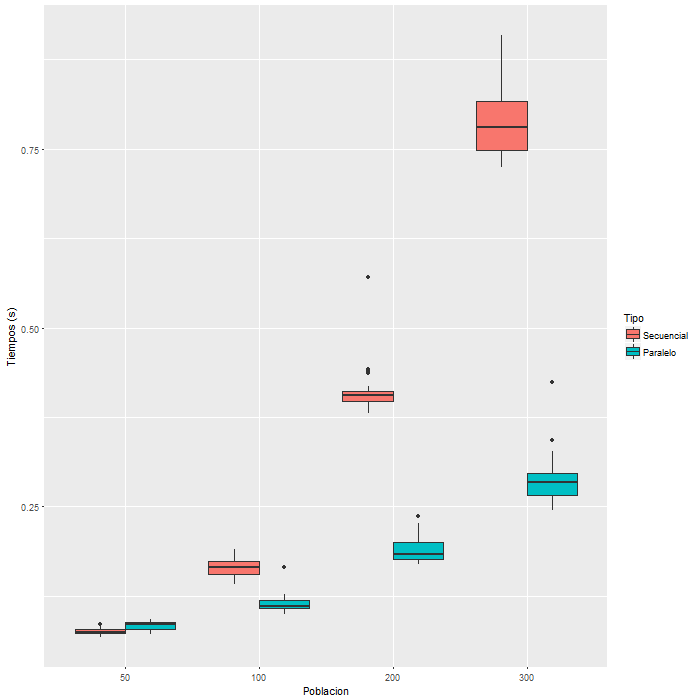
\includegraphics[width=0.7\linewidth]{ambos}
\caption{Tiempos de corrida respecto a cantidad de variables iniciales.}
\label{fig:ambos}
\end{figure}



\end{document}